
\outline{3}{Exercise 12.10}
\subsubsection*{Exercise 12.10}

\textit{What would happen if the space of the forest fire propagation were 1-D
or 3-D? Conduct the renormalization group analysis to see what happens in those
cases.}

\vspace{5mm}
\textbf{One-diomensional case:}

\vspace{5mm}
The probability of percolation for one cell is the probability of that cell
assume value $1$:
\begin{equation}
  p_1 = q.
\end{equation}

Expand our group to two cells, the percolation proccess will occur only if the
two cells assume value $1$:
\begin{equation}
  p_2 = {p_1}^2.
\end{equation}

In fact, we can generalize the previous equation to:
\begin{equation}
  p_{s+1} = {p_s}^2,
\end{equation}

and conclude that if one cell in our system assume $0$, the propagation will be
stopped.

\vspace{5mm}
\textbf{Three-diomensional case:}

\vspace{5mm}
Despite the three dimensions of cells, the probability of percolation for one
cell is equal to previous case:
\begin{equation}
  p_1 = q.
\end{equation}

In this case is actually easier to list possibilities that don\textquotesingle t
allow percolation. The number of possible configurations for the renormalization
group analysis made of $2\times2\times2$ cells is:
\begin{equation}
  S = 256, \qquad S = k^{L^{D}}, \quad k = L = 2, \quad D = 3.
\end{equation}

Since cells have Moore\textquotesingle s neighborhood, any cell is neighbor to
the other cells. Imagine the renormalization group as two $2\times2$ planes, and
the percolation proccess from one plane to another. Possibilities that cells are
all in one of these two planes prevents the percolation process. To list then:

\vspace{5mm}
1 from empty cells; \\
2 from 4 cells filled; \\
8 from 3 cells filled; \\
8 from 1 cell filled; \\
12 from 2 cells filled;

\vspace{5mm}
A total of 31 possibilities, that leads to the relation of possibilities in
which we have percolation proccess and total number of possibilities:
\begin{equation}
  \frac{225}{256}
\end{equation}

The critical percolation threshold is given by:
\begin{equation}
  \begin{aligned}
    p_c = { } & 1 - \\
              & 1 \times (1-p_c)^8 - \\
              & 2 \times {p_c}^4 (1-p_c)^4 - \\
              & 8 \times {p_c}^3 (1-p_c)^5 - \\
              & 8 \times p_c (1-p_c)^7 - \\
              & 12 \times {p_c}^2 (1-p_c)^6.
  \end{aligned}
\end{equation}

And the cobweb plot for that equation is:
\begin{figure}[h]
  \centering
  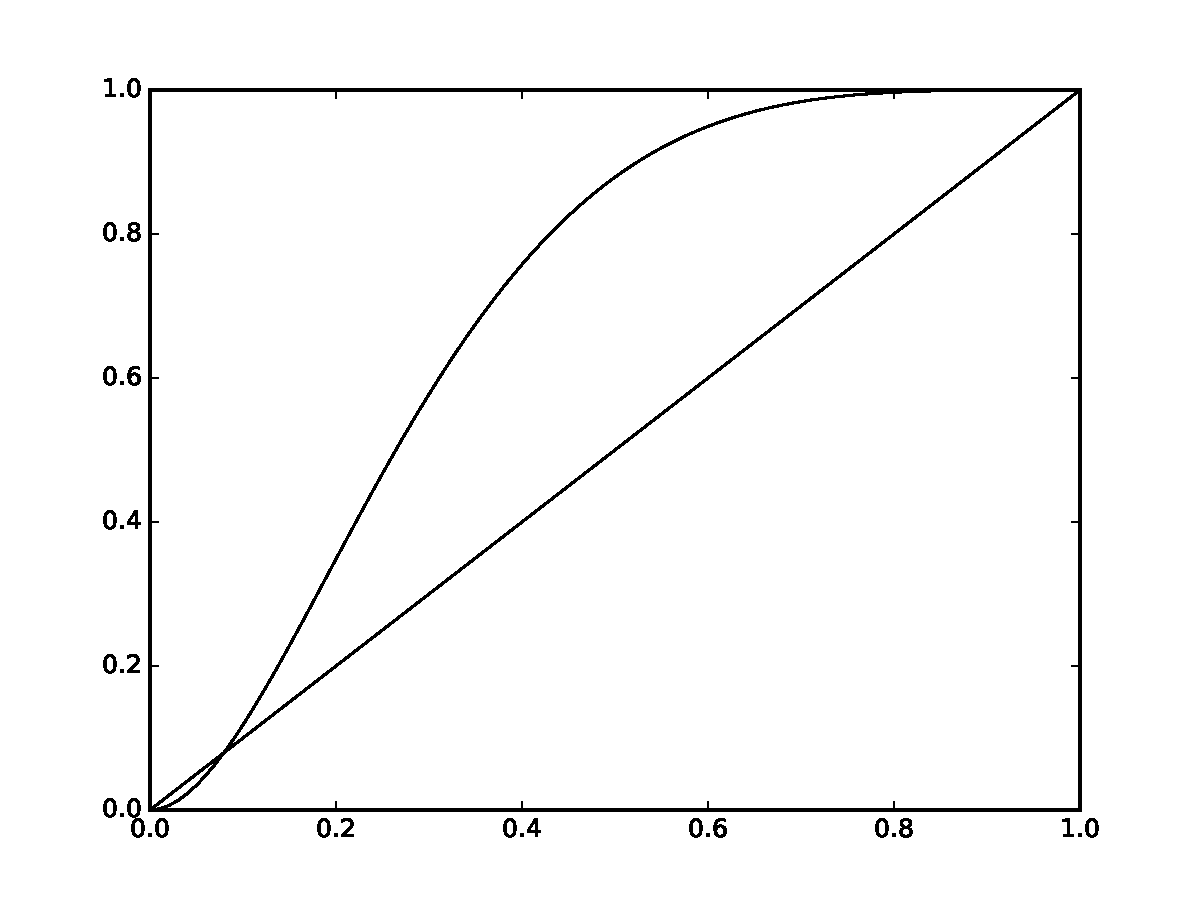
\includegraphics[width=0.75\textwidth]{./figures/12.10-cobweb-plot-for-3-dimensional.pdf}
  \caption{\texttt{12.10-cobweb-plot-for-3-dimensional.py}}
\end{figure}

In which is easy to see two asymptotic states possible, $p_\infty = 0$ and
$p_\infty = 1$ (the cobweb plot is about relations over scale, not about
dynamics over time). There is an unstable equilibrium point around $p = 0.1$.
The approximate value is:
\begin{equation}
  p \approx 0.0794325.
\end{equation}

\textbf{Comparnison of cases:}
\vspace{5mm}

The relation of possibilities in which we have percolation proccess and total
number of possibilities for the 1-D, 2-D and 3-D are, respectively:
\begin{equation}
  \frac{1}{4} < \frac{9}{16} < \frac{225}{256}.
\end{equation}

For one-dimensional systems, the critical percolation threshold is $100 \%$,
since all cells must assume $1$ to percolation to occur. For two-dimensional,
the threshold is $38 \%$. Finally, for three-dimensional systems, the threshold
is under $8 \%$.

\vspace{5mm}
From this we can conclude that as we increase the number of dimensions, we
increase the susceptibility to percolation.
